% 建议使用 XeLaTeX 或 LuaLaTeX 编译(中文与公式支持更佳)
\documentclass[UTF8,zihao=-4]{ctexart}

% 版式与常用宏包
\usepackage[a4paper,margin=2.5cm]{geometry}
\usepackage{amsmath, amssymb, amsthm}
\usepackage{bm}
\usepackage{hyperref}
\usepackage{graphicx}
\usepackage{caption}
\usepackage{listings}
\usepackage{xcolor}
\graphicspath{{figures/}}

% 代码样式
\lstdefinestyle{code}{
  basicstyle=\ttfamily\small,
  numbers=left,
  numberstyle=\tiny,
  numbersep=8pt,
  keywordstyle=\color{blue},
  commentstyle=\color{teal!70!black},
  stringstyle=\color{orange!70!black},
  showstringspaces=false,
  breaklines=true,
  frame=single,
  framerule=0.3pt,
  rulecolor=\color{black!15}
}
\lstset{style=code}

\title{线性回归:原理、公式、应用与实战}
\author{}
\date{\today}

\begin{document}
\maketitle
\tableofcontents

\section{引言}
线性回归(Linear Regression)是监督学习中最基础的回归算法之一,旨在学习输入特征与连续目标变量之间的线性关系。凭借可解释性强、训练高效、闭式解可得等优点,线性回归在工程与科研中广泛用作基线模型与快速验证工具。

\section{原理与公式}
\subsection{模型假设与表示}
给定特征向量 \(\mathbf{x} \in \mathbb{R}^d\),线性回归假设目标 \(y\) 满足
\begin{equation}
    \hat{y} = f(\mathbf{x}) = \mathbf{w}^\top \mathbf{x} + b,\quad \mathbf{w} \in \mathbb{R}^d,\; b \in \mathbb{R}.
\end{equation}
将偏置并入权向量(令 \(\tilde{\mathbf{x}}=[\mathbf{x};1]\)、\(\tilde{\mathbf{w}}=[\mathbf{w};b]\)),可写为 \(\hat{y}=\tilde{\mathbf{w}}^\top \tilde{\mathbf{x}}\)。

\subsection{矩阵形式}
给定样本矩阵 \(\mathbf{X}\in\mathbb{R}^{n\times d}\) 与标签向量 \(\mathbf{y}\in\mathbb{R}^{n}\),预测向量 \(\hat{\mathbf{y}}=\mathbf{X}\mathbf{w}+b\mathbf{1}\)。引入增广矩阵 \(\tilde{\mathbf{X}}=[\mathbf{X}\,\,\mathbf{1}]\) 与 \(\tilde{\mathbf{w}}=[\mathbf{w};b]\),则 \(\hat{\mathbf{y}}=\tilde{\mathbf{X}}\tilde{\mathbf{w}}\)。

\subsection{损失函数(最小二乘)}
常用目标为均方误差(MSE):
\begin{equation}
    \mathcal{L}(\tilde{\mathbf{w}}) = \frac{1}{2n} \lVert \tilde{\mathbf{X}}\tilde{\mathbf{w}} - \mathbf{y} \rVert_2^2.
\end{equation}

\subsection{闭式解(普通最小二乘 OLS)}
当 \(\tilde{\mathbf{X}}^\top\tilde{\mathbf{X}}\) 可逆时,最优解为
\begin{equation}
    \tilde{\mathbf{w}}^* = \big(\tilde{\mathbf{X}}^\top\tilde{\mathbf{X}}\big)^{-1}\tilde{\mathbf{X}}^\top\mathbf{y}.
\end{equation}
在数值实现中常采用 QR 分解或 SVD 提升稳定性。

\subsection{梯度下降(可选)}
亦可用一阶优化:
\begin{align}
    \nabla_{\tilde{\mathbf{w}}} \mathcal{L} &= \frac{1}{n} \tilde{\mathbf{X}}^\top\big(\tilde{\mathbf{X}}\tilde{\mathbf{w}} - \mathbf{y}\big),\\
    \tilde{\mathbf{w}} &\leftarrow \tilde{\mathbf{w}} - \eta\, \nabla_{\tilde{\mathbf{w}}} \mathcal{L},
\end{align}
其中 \(\eta\) 为学习率。

\subsection{正则化(可选)}
以岭回归(L2)为例:
\begin{equation}
    \min_{\tilde{\mathbf{w}}}\; \frac{1}{2n}\lVert \tilde{\mathbf{X}}\tilde{\mathbf{w}}-\mathbf{y}\rVert_2^2 + \frac{\lambda}{2}\lVert \mathbf{w}\rVert_2^2.
\end{equation}
其闭式解为 \(\tilde{\mathbf{w}}^* = (\tilde{\mathbf{X}}^\top\tilde{\mathbf{X}} + \lambda\mathbf{I})^{-1}\tilde{\mathbf{X}}^\top\mathbf{y}\)。

\section{应用场景与使用要点}
\begin{itemize}
  \item \textbf{数值预测与趋势建模}:如房价、销量、温度等连续变量的估计。
  \item \textbf{可解释性基线}:提供特征重要性线索(系数大小与符号),便于快速决策与沟通。
  \item \textbf{工程要点}:特征缩放、异常值处理、多重共线性诊断、交叉验证选择正则强度等。
\end{itemize}

\section{Python 实战:闭式解拟合与可视化}
下面的示例将:
\begin{enumerate}
  \item 生成一维线性数据并加入噪声;
  \item 通过增广矩阵使用普通最小二乘闭式解求参;
  \item 绘制散点与拟合直线,并保存到 \texttt{figures/linear\_regression\_fit.png}。
\end{enumerate}

\begin{lstlisting}[language=Python,caption={linear_regression_closed_form.py}]
import os
import numpy as np
import matplotlib.pyplot as plt

np.random.seed(42)

# 1) 生成数据: y = 3x + 2 + 噪声
n = 80
X = np.linspace(-3, 3, n).reshape(-1, 1)
true_w, true_b = 3.0, 2.0
y = true_w * X[:, 0] + true_b + np.random.normal(0, 1.0, size=n)

# 2) 增广矩阵与闭式解
X_aug = np.hstack([X, np.ones((n, 1))])  # [x, 1]
theta = np.linalg.pinv(X_aug.T @ X_aug) @ X_aug.T @ y
w_hat, b_hat = theta[0], theta[1]

# 3) 可视化并保存
fig, ax = plt.subplots(figsize=(6, 4))
ax.scatter(X[:, 0], y, s=18, alpha=0.7, label='data')
xx = np.linspace(X.min(), X.max(), 200)
yy = w_hat * xx + b_hat
ax.plot(xx, yy, color='crimson', lw=2.0, label=f'fit: y={w_hat:.2f}x+{b_hat:.2f}')
ax.set_xlabel('x')
ax.set_ylabel('y')
ax.legend()
ax.set_title('Linear Regression (Closed-form OLS)')

os.makedirs('figures', exist_ok=True)
out_path = os.path.join('figures', 'linear_regression_fit.png')
plt.tight_layout()
plt.savefig(out_path, dpi=160)
print('saved to', out_path)
\end{lstlisting}

\section{运行效果}
图~\ref{fig:fit} 展示了闭式解拟合得到的直线与带噪声数据散点。

\begin{figure}[h]
  \centering
  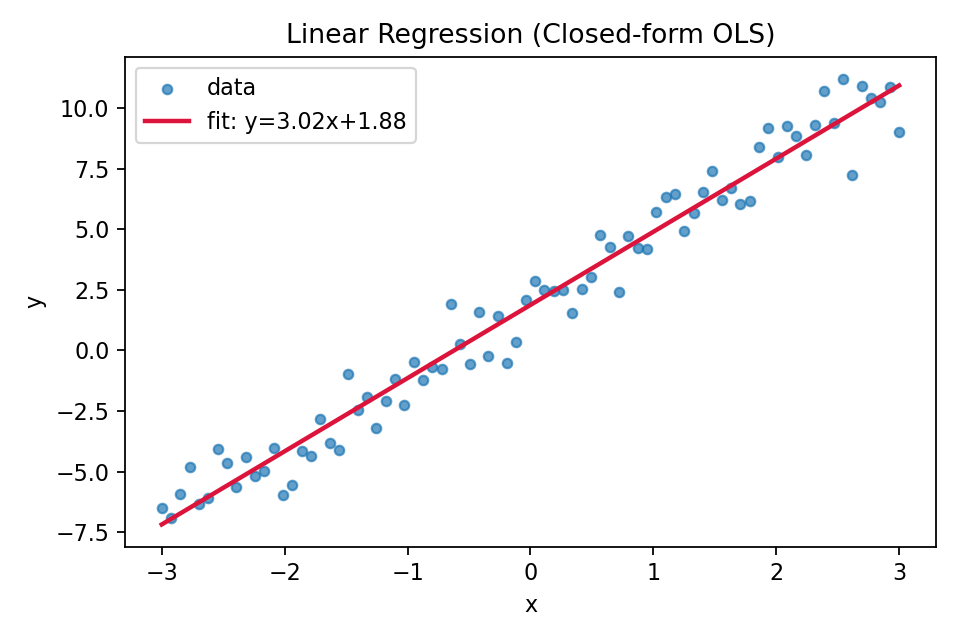
\includegraphics[width=0.75\linewidth]{linear_regression_fit.png}
  \caption{线性回归拟合效果示意(合成数据)}
  \label{fig:fit}
\end{figure}

\section{小结}
线性回归以其简洁与高效成为常见的回归基线方法。实践中应注意数据尺度、异常值与共线性,并通过交叉验证选择正则化强度,以获得稳健的泛化能力与可解释性。

\end{document}

